\documentclass[1p]{elsarticle_modified}
%\bibliographystyle{elsarticle-num}

%\usepackage[colorlinks]{hyperref}
%\usepackage{abbrmath_seonhwa} %\Abb, \Ascr, \Acal ,\Abf, \Afrak
\usepackage{amsfonts}
\usepackage{amssymb}
\usepackage{amsmath}
\usepackage{amsthm}
\usepackage{scalefnt}
\usepackage{amsbsy}
\usepackage{kotex}
\usepackage{caption}
\usepackage{subfig}
\usepackage{color}
\usepackage{graphicx}
\usepackage{xcolor} %% white, black, red, green, blue, cyan, magenta, yellow
\usepackage{float}
\usepackage{setspace}
\usepackage{hyperref}

\usepackage{tikz}
\usetikzlibrary{arrows}

\usepackage{multirow}
\usepackage{array} % fixed length table
\usepackage{hhline}

%%%%%%%%%%%%%%%%%%%%%
\makeatletter
\renewcommand*\env@matrix[1][\arraystretch]{%
	\edef\arraystretch{#1}%
	\hskip -\arraycolsep
	\let\@ifnextchar\new@ifnextchar
	\array{*\c@MaxMatrixCols c}}
\makeatother %https://tex.stackexchange.com/questions/14071/how-can-i-increase-the-line-spacing-in-a-matrix
%%%%%%%%%%%%%%%

\usepackage[normalem]{ulem}

\newcommand{\msout}[1]{\ifmmode\text{\sout{\ensuremath{#1}}}\else\sout{#1}\fi}
%SOURCE: \msout is \stkout macro in https://tex.stackexchange.com/questions/20609/strikeout-in-math-mode

\newcommand{\cancel}[1]{
	\ifmmode
	{\color{red}\msout{#1}}
	\else
	{\color{red}\sout{#1}}
	\fi
}

\newcommand{\add}[1]{
	{\color{blue}\uwave{#1}}
}

\newcommand{\replace}[2]{
	\ifmmode
	{\color{red}\msout{#1}}{\color{blue}\uwave{#2}}
	\else
	{\color{red}\sout{#1}}{\color{blue}\uwave{#2}}
	\fi
}

\newcommand{\Sol}{\mathcal{S}} %segment
\newcommand{\D}{D} %diagram
\newcommand{\A}{\mathcal{A}} %arc


%%%%%%%%%%%%%%%%%%%%%%%%%%%%%5 test

\def\sl{\operatorname{\textup{SL}}(2,\Cbb)}
\def\psl{\operatorname{\textup{PSL}}(2,\Cbb)}
\def\quan{\mkern 1mu \triangleright \mkern 1mu}

\theoremstyle{definition}
\newtheorem{thm}{Theorem}[section]
\newtheorem{prop}[thm]{Proposition}
\newtheorem{lem}[thm]{Lemma}
\newtheorem{ques}[thm]{Question}
\newtheorem{cor}[thm]{Corollary}
\newtheorem{defn}[thm]{Definition}
\newtheorem{exam}[thm]{Example}
\newtheorem{rmk}[thm]{Remark}
\newtheorem{alg}[thm]{Algorithm}

\newcommand{\I}{\sqrt{-1}}
\begin{document}

%\begin{frontmatter}
%
%\title{Boundary parabolic representations of knots up to 8 crossings}
%
%%% Group authors per affiliation:
%\author{Yunhi Cho} 
%\address{Department of Mathematics, University of Seoul, Seoul, Korea}
%\ead{yhcho@uos.ac.kr}
%
%
%\author{Seonhwa Kim} %\fnref{s_kim}}
%\address{Center for Geometry and Physics, Institute for Basic Science, Pohang, 37673, Korea}
%\ead{ryeona17@ibs.re.kr}
%
%\author{Hyuk Kim}
%\address{Department of Mathematical Sciences, Seoul National University, Seoul 08826, Korea}
%\ead{hyukkim@snu.ac.kr}
%
%\author{Seokbeom Yoon}
%\address{Department of Mathematical Sciences, Seoul National University, Seoul, 08826,  Korea}
%\ead{sbyoon15@snu.ac.kr}
%
%\begin{abstract}
%We find all boundary parabolic representation of knots up to 8 crossings.
%
%\end{abstract}
%\begin{keyword}
%    \MSC[2010] 57M25 
%\end{keyword}
%
%\end{frontmatter}

%\linenumbers
%\tableofcontents
%
\newcommand\colored[1]{\textcolor{white}{\rule[-0.35ex]{0.8em}{1.4ex}}\kern-0.8em\color{red} #1}%
%\newcommand\colored[1]{\textcolor{white}{ #1}\kern-2.17ex	\textcolor{white}{ #1}\kern-1.81ex	\textcolor{white}{ #1}\kern-2.15ex\color{red}#1	}

{\Large $\underline{12n_{0402}~(K12n_{0402})}$}

\setlength{\tabcolsep}{10pt}
\renewcommand{\arraystretch}{1.6}
\vspace{1cm}\begin{tabular}{m{100pt}>{\centering\arraybackslash}m{274pt}}
\multirow{5}{120pt}{
	\centering
	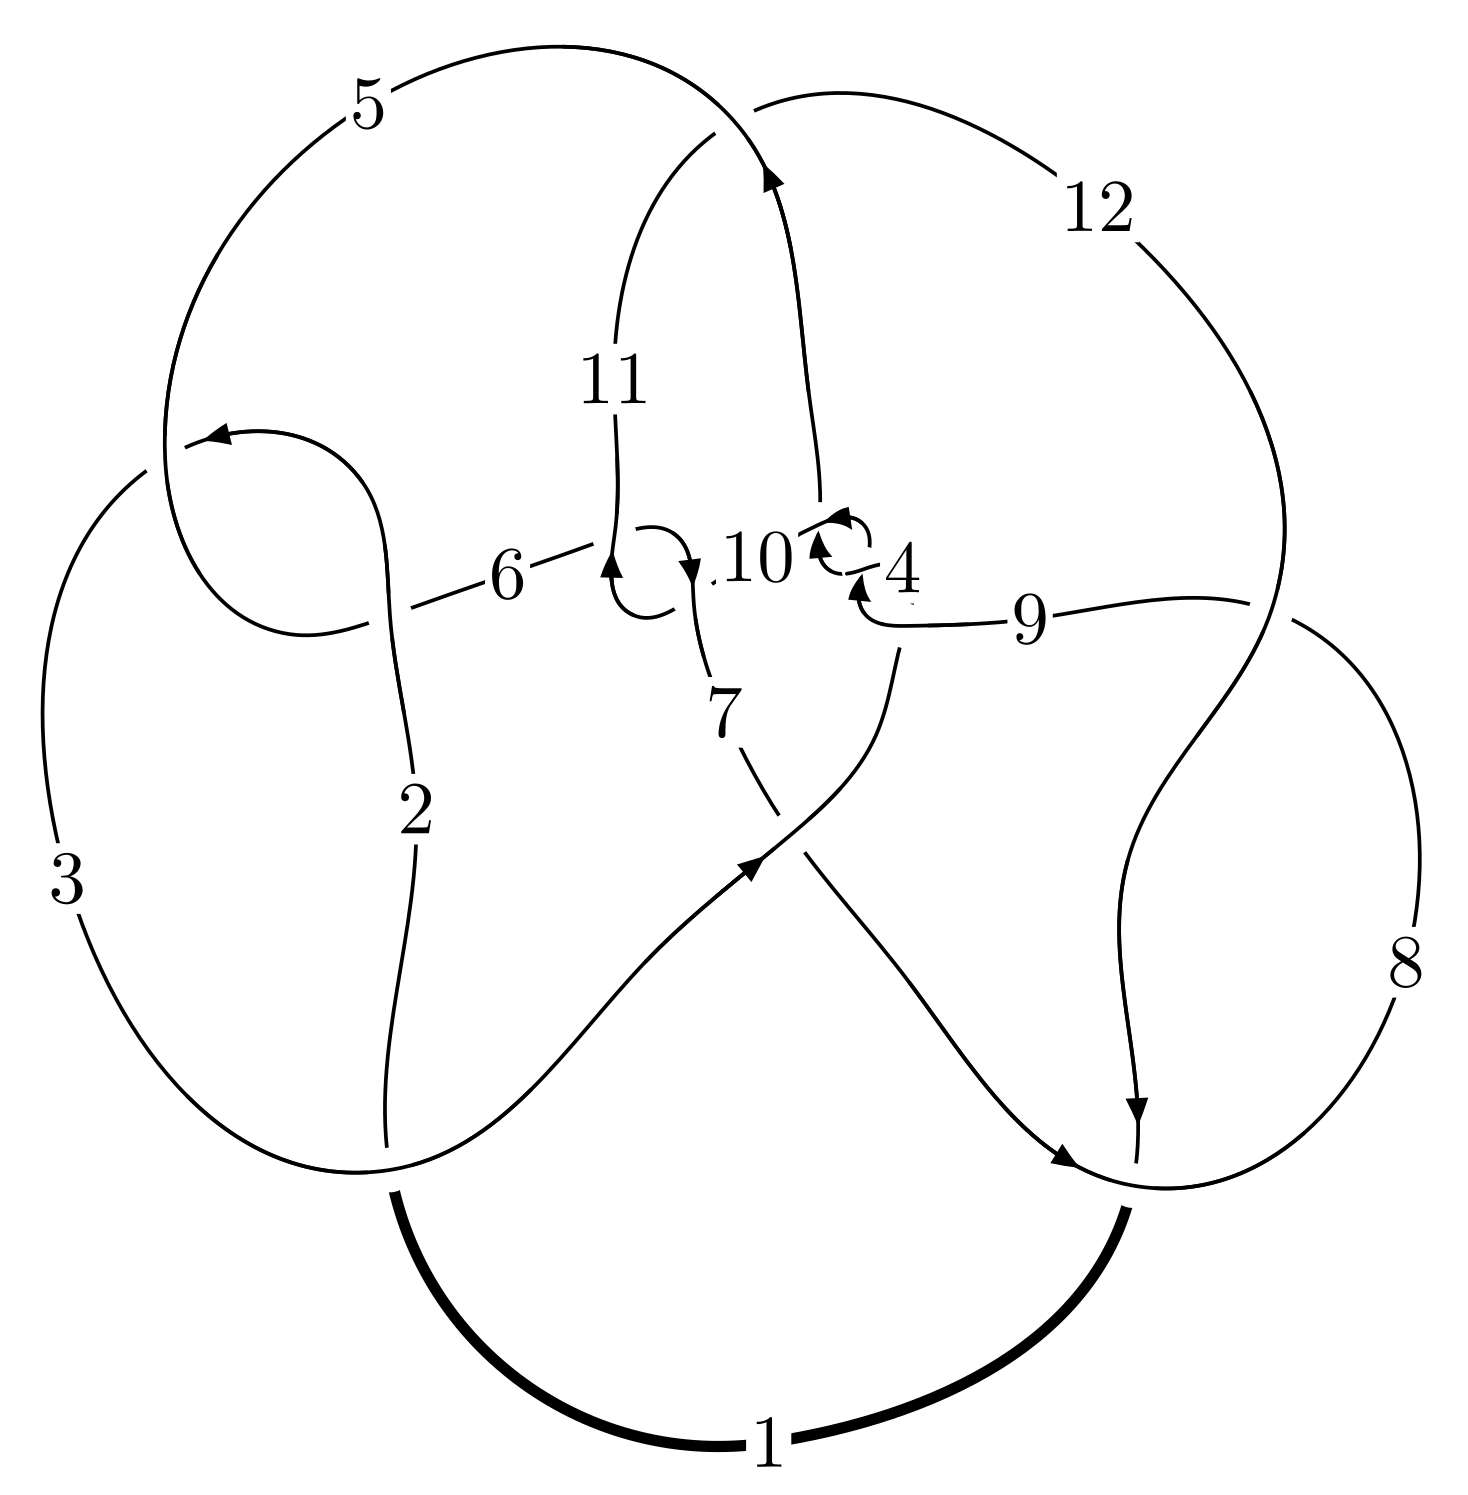
\includegraphics[width=112pt]{../../../GIT/diagram.site/Diagrams/png/2491_12n_0402.png}\\
\ \ \ A knot diagram\footnotemark}&
\allowdisplaybreaks
\textbf{Linearized knot diagam} \\
\cline{2-2}
 &
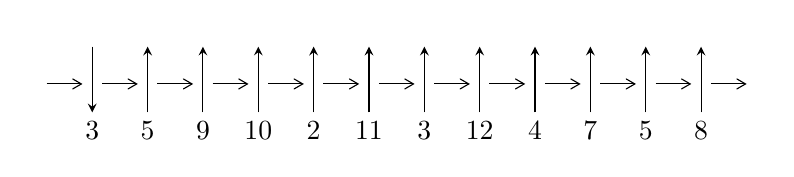
\begin{tikzpicture}[x=20pt, y=17pt]
	% nodes
	\node (C0) at (0, 0) {};
	\node (C1) at (1, 0) {};
	\node (C1U) at (1, +1) {};
	\node (C1D) at (1, -1) {3};

	\node (C2) at (2, 0) {};
	\node (C2U) at (2, +1) {};
	\node (C2D) at (2, -1) {5};

	\node (C3) at (3, 0) {};
	\node (C3U) at (3, +1) {};
	\node (C3D) at (3, -1) {9};

	\node (C4) at (4, 0) {};
	\node (C4U) at (4, +1) {};
	\node (C4D) at (4, -1) {10};

	\node (C5) at (5, 0) {};
	\node (C5U) at (5, +1) {};
	\node (C5D) at (5, -1) {2};

	\node (C6) at (6, 0) {};
	\node (C6U) at (6, +1) {};
	\node (C6D) at (6, -1) {11};

	\node (C7) at (7, 0) {};
	\node (C7U) at (7, +1) {};
	\node (C7D) at (7, -1) {3};

	\node (C8) at (8, 0) {};
	\node (C8U) at (8, +1) {};
	\node (C8D) at (8, -1) {12};

	\node (C9) at (9, 0) {};
	\node (C9U) at (9, +1) {};
	\node (C9D) at (9, -1) {4};

	\node (C10) at (10, 0) {};
	\node (C10U) at (10, +1) {};
	\node (C10D) at (10, -1) {7};

	\node (C11) at (11, 0) {};
	\node (C11U) at (11, +1) {};
	\node (C11D) at (11, -1) {5};

	\node (C12) at (12, 0) {};
	\node (C12U) at (12, +1) {};
	\node (C12D) at (12, -1) {8};
	\node (C13) at (13, 0) {};

	% arrows
	\draw[->,>={angle 60}]
	(C0) edge (C1) (C1) edge (C2) (C2) edge (C3) (C3) edge (C4) (C4) edge (C5) (C5) edge (C6) (C6) edge (C7) (C7) edge (C8) (C8) edge (C9) (C9) edge (C10) (C10) edge (C11) (C11) edge (C12) (C12) edge (C13) ;	\draw[->,>=stealth]
	(C1U) edge (C1D) (C2D) edge (C2U) (C3D) edge (C3U) (C4D) edge (C4U) (C5D) edge (C5U) (C6D) edge (C6U) (C7D) edge (C7U) (C8D) edge (C8U) (C9D) edge (C9U) (C10D) edge (C10U) (C11D) edge (C11U) (C12D) edge (C12U) ;
	\end{tikzpicture} \\
\hhline{~~} \\& 
\textbf{Solving Sequence} \\ \cline{2-2} 
 &
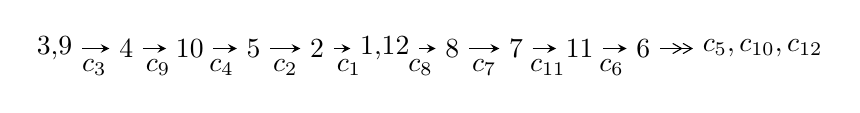
\begin{tikzpicture}[x=23pt, y=7pt]
	% node
	\node (A0) at (-1/8, 0) {3,9};
	\node (A1) at (1, 0) {4};
	\node (A2) at (2, 0) {10};
	\node (A3) at (3, 0) {5};
	\node (A4) at (4, 0) {2};
	\node (A5) at (81/16, 0) {1,12};
	\node (A6) at (49/8, 0) {8};
	\node (A7) at (57/8, 0) {7};
	\node (A8) at (65/8, 0) {11};
	\node (A9) at (73/8, 0) {6};
	\node (C1) at (1/2, -1) {$c_{3}$};
	\node (C2) at (3/2, -1) {$c_{9}$};
	\node (C3) at (5/2, -1) {$c_{4}$};
	\node (C4) at (7/2, -1) {$c_{2}$};
	\node (C5) at (9/2, -1) {$c_{1}$};
	\node (C6) at (45/8, -1) {$c_{8}$};
	\node (C7) at (53/8, -1) {$c_{7}$};
	\node (C8) at (61/8, -1) {$c_{11}$};
	\node (C9) at (69/8, -1) {$c_{6}$};
	\node (A10) at (11, 0) {$c_{5},c_{10},c_{12}$};

	% edge
	\draw[->,>=stealth]	
	(A0) edge (A1) (A1) edge (A2) (A2) edge (A3) (A3) edge (A4) (A4) edge (A5) (A5) edge (A6) (A6) edge (A7) (A7) edge (A8) (A8) edge (A9) ;
	\draw[->>,>={angle 60}]	
	(A9) edge (A10);
\end{tikzpicture} \\ 

\end{tabular} \\

\footnotetext{
The image of knot diagram is generated by the software ``\textbf{Draw programme}" developed by Andrew Bartholomew(\url{http://www.layer8.co.uk/maths/draw/index.htm\#Running-draw}), where we modified some parts for our purpose(\url{https://github.com/CATsTAILs/LinksPainter}).
}\phantom \\ \newline 
\centering \textbf{Ideals for irreducible components\footnotemark of $X_{\text{par}}$} 
 
\begin{align*}
I^u_{1}&=\langle 
- u^9+2 u^8+3 u^7-4 u^6-6 u^5-2 u^4+9 u^3+4 u^2+b-1,\\
\phantom{I^u_{1}}&\phantom{= \langle  }u^9- u^8-3 u^7- u^6+5 u^5+9 u^4-4 u^3-6 u^2+2 a-5 u+1,\\
\phantom{I^u_{1}}&\phantom{= \langle  }u^{10}-3 u^9- u^8+7 u^7+3 u^6-5 u^5-14 u^4+6 u^3+7 u^2+3 u-2\rangle \\
I^u_{2}&=\langle 
- u^5+3 u^3+b- u+1,\;u^6-4 u^4+4 u^2+a,\;u^8-5 u^6+7 u^4-2 u^2+1\rangle \\
I^u_{3}&=\langle 
b+1,\;a^2+a+2,\;u+1\rangle \\
\\
\end{align*}
\raggedright * 3 irreducible components of $\dim_{\mathbb{C}}=0$, with total 20 representations.\\
\footnotetext{All coefficients of polynomials are rational numbers. But the coefficients are sometimes approximated in decimal forms when there is not enough margin.}
\newpage
\renewcommand{\arraystretch}{1}
\centering \section*{I. $I^u_{1}= \langle - u^9+2 u^8+\cdots+b-1,\;u^9- u^8+\cdots+2 a+1,\;u^{10}-3 u^9+\cdots+3 u-2 \rangle$}
\flushleft \textbf{(i) Arc colorings}\\
\begin{tabular}{m{7pt} m{180pt} m{7pt} m{180pt} }
\flushright $a_{3}=$&$\begin{pmatrix}1\\0\end{pmatrix}$ \\
\flushright $a_{9}=$&$\begin{pmatrix}0\\u\end{pmatrix}$ \\
\flushright $a_{4}=$&$\begin{pmatrix}1\\- u^2\end{pmatrix}$ \\
\flushright $a_{10}=$&$\begin{pmatrix}u\\- u^3+u\end{pmatrix}$ \\
\flushright $a_{5}=$&$\begin{pmatrix}- u^2+1\\u^4-2 u^2\end{pmatrix}$ \\
\flushright $a_{2}=$&$\begin{pmatrix}- u^6+3 u^4-2 u^2+1\\u^8-4 u^6+4 u^4\end{pmatrix}$ \\
\flushright $a_{1}=$&$\begin{pmatrix}u^8-5 u^6+7 u^4-2 u^2+1\\u^8-4 u^6+4 u^4\end{pmatrix}$ \\
\flushright $a_{12}=$&$\begin{pmatrix}-\frac{1}{2} u^9+\frac{1}{2} u^8+\cdots+\frac{5}{2} u-\frac{1}{2}\\u^9-2 u^8-3 u^7+4 u^6+6 u^5+2 u^4-9 u^3-4 u^2+1\end{pmatrix}$ \\
\flushright $a_{8}=$&$\begin{pmatrix}\frac{1}{2} u^9-\frac{1}{2} u^8+\cdots-\frac{1}{2} u+\frac{1}{2}\\u^9- u^8-4 u^7+u^6+7 u^5+4 u^4-6 u^3-4 u^2+1\end{pmatrix}$ \\
\flushright $a_{7}=$&$\begin{pmatrix}-\frac{1}{2} u^9+\frac{1}{2} u^8+\cdots-\frac{1}{2} u-\frac{1}{2}\\u^9- u^8-4 u^7+u^6+7 u^5+4 u^4-6 u^3-4 u^2+1\end{pmatrix}$ \\
\flushright $a_{11}=$&$\begin{pmatrix}\frac{3}{2} u^9-\frac{5}{2} u^8+\cdots-\frac{3}{2} u+\frac{5}{2}\\- u^9+3 u^8+3 u^7-8 u^6-6 u^5+2 u^4+8 u^3+4 u^2+u-1\end{pmatrix}$ \\
\flushright $a_{6}=$&$\begin{pmatrix}3 u^9-4 u^8-7 u^7+5 u^6+5 u^5+9 u^4-6 u^3-4 u^2-3 u+1\\-8 u^9+8 u^8+32 u^7-9 u^6-56 u^5-32 u^4+48 u^3+37 u^2+6 u-8\end{pmatrix}$\\&\end{tabular}
\flushleft \textbf{(ii) Obstruction class $= -1$}\\~\\
\flushleft \textbf{(iii) Cusp Shapes $= -4 u^9+6 u^8+12 u^7-6 u^6-22 u^5-22 u^4+22 u^3+20 u^2+18 u+10$}\\~\\
\newpage\renewcommand{\arraystretch}{1}
\flushleft \textbf{(iv) u-Polynomials at the component}\newline \\
\begin{tabular}{m{50pt}|m{274pt}}
Crossings & \hspace{64pt}u-Polynomials at each crossing \\
\hline $$\begin{aligned}c_{1}\end{aligned}$$&$\begin{aligned}
&u^{10}+49 u^9+\cdots-2401 u+64
\end{aligned}$\\
\hline $$\begin{aligned}c_{2},c_{5}\end{aligned}$$&$\begin{aligned}
&u^{10}+u^9+\cdots-9 u-8
\end{aligned}$\\
\hline $$\begin{aligned}c_{3},c_{4},c_{9}\end{aligned}$$&$\begin{aligned}
&u^{10}-3 u^9- u^8+7 u^7+3 u^6-5 u^5-14 u^4+6 u^3+7 u^2+3 u-2
\end{aligned}$\\
\hline $$\begin{aligned}c_{6},c_{8},c_{10}\\c_{12}\end{aligned}$$&$\begin{aligned}
&u^{10}+13 u^8+2 u^7+48 u^6+30 u^5+20 u^4+14 u^3- u^2+2 u-1
\end{aligned}$\\
\hline $$\begin{aligned}c_{7},c_{11}\end{aligned}$$&$\begin{aligned}
&u^{10}-2 u^9+\cdots-54 u-29
\end{aligned}$\\
\hline
\end{tabular}\\~\\
\newpage\renewcommand{\arraystretch}{1}
\flushleft \textbf{(v) Riley Polynomials at the component}\newline \\
\begin{tabular}{m{50pt}|m{274pt}}
Crossings & \hspace{64pt}Riley Polynomials at each crossing \\
\hline $$\begin{aligned}c_{1}\end{aligned}$$&$\begin{aligned}
&y^{10}-535 y^9+\cdots-3422273 y+4096
\end{aligned}$\\
\hline $$\begin{aligned}c_{2},c_{5}\end{aligned}$$&$\begin{aligned}
&y^{10}+49 y^9+\cdots-2401 y+64
\end{aligned}$\\
\hline $$\begin{aligned}c_{3},c_{4},c_{9}\end{aligned}$$&$\begin{aligned}
&y^{10}-11 y^9+\cdots-37 y+4
\end{aligned}$\\
\hline $$\begin{aligned}c_{6},c_{8},c_{10}\\c_{12}\end{aligned}$$&$\begin{aligned}
&y^{10}+26 y^9+\cdots-2 y+1
\end{aligned}$\\
\hline $$\begin{aligned}c_{7},c_{11}\end{aligned}$$&$\begin{aligned}
&y^{10}+110 y^9+\cdots-23448 y+841
\end{aligned}$\\
\hline
\end{tabular}\\~\\
\newpage\flushleft \textbf{(vi) Complex Volumes and Cusp Shapes}
$$\begin{array}{c|c|c}  
\text{Solutions to }I^u_{1}& \I (\text{vol} + \sqrt{-1}CS) & \text{Cusp shape}\\
 \hline 
\begin{aligned}
u &= -0.632414 + 0.947419 I \\
a &= \phantom{-}2.18175 - 1.13028 I \\
b &= \phantom{-}2.28217 - 0.07300 I\end{aligned}
 & \phantom{-}15.8724 - 3.1297 I & \phantom{-}7.30319 + 2.05885 I \\ \hline\begin{aligned}
u &= -0.632414 - 0.947419 I \\
a &= \phantom{-}2.18175 + 1.13028 I \\
b &= \phantom{-}2.28217 + 0.07300 I\end{aligned}
 & \phantom{-}15.8724 + 3.1297 I & \phantom{-}7.30319 - 2.05885 I \\ \hline\begin{aligned}
u &= -0.481550 + 0.474579 I \\
a &= -0.609360 + 0.497018 I \\
b &= -0.743164 - 0.230554 I\end{aligned}
 & -1.67643 - 1.67312 I & \phantom{-}8.34167 + 5.35276 I \\ \hline\begin{aligned}
u &= -0.481550 - 0.474579 I \\
a &= -0.609360 - 0.497018 I \\
b &= -0.743164 + 0.230554 I\end{aligned}
 & -1.67643 + 1.67312 I & \phantom{-}8.34167 - 5.35276 I \\ \hline\begin{aligned}
u &= -1.44882\phantom{ +0.000000I} \\
a &= \phantom{-}0.519822\phantom{ +0.000000I} \\
b &= \phantom{-}0.723841\phantom{ +0.000000I}\end{aligned}
 & \phantom{-}6.49727\phantom{ +0.000000I} & \phantom{-}15.2060\phantom{ +0.000000I} \\ \hline\begin{aligned}
u &= \phantom{-}1.53180 + 0.11762 I \\
a &= -0.119445 - 0.373636 I \\
b &= -0.797864 + 0.675313 I\end{aligned}
 & \phantom{-}5.05958 + 3.70571 I & \phantom{-}13.2497 - 5.2095 I \\ \hline\begin{aligned}
u &= \phantom{-}1.53180 - 0.11762 I \\
a &= -0.119445 + 0.373636 I \\
b &= -0.797864 - 0.675313 I\end{aligned}
 & \phantom{-}5.05958 - 3.70571 I & \phantom{-}13.2497 + 5.2095 I \\ \hline\begin{aligned}
u &= \phantom{-}0.358246\phantom{ +0.000000I} \\
a &= \phantom{-}0.785999\phantom{ +0.000000I} \\
b &= \phantom{-}0.146927\phantom{ +0.000000I}\end{aligned}
 & \phantom{-}0.511729\phantom{ +0.000000I} & \phantom{-}19.5320\phantom{ +0.000000I} \\ \hline\begin{aligned}
u &= \phantom{-}1.62745 + 0.32233 I \\
a &= \phantom{-}0.64414 + 1.30973 I \\
b &= \phantom{-}2.32347 + 0.23227 I\end{aligned}
 & -16.1803 + 7.8809 I & \phantom{-}9.73645 - 2.75764 I \\ \hline\begin{aligned}
u &= \phantom{-}1.62745 - 0.32233 I \\
a &= \phantom{-}0.64414 - 1.30973 I \\
b &= \phantom{-}2.32347 - 0.23227 I\end{aligned}
 & -16.1803 - 7.8809 I & \phantom{-}9.73645 + 2.75764 I\\
 \hline 
 \end{array}$$\newpage\newpage\renewcommand{\arraystretch}{1}
\centering \section*{II. $I^u_{2}= \langle - u^5+3 u^3+b- u+1,\;u^6-4 u^4+4 u^2+a,\;u^8-5 u^6+7 u^4-2 u^2+1 \rangle$}
\flushleft \textbf{(i) Arc colorings}\\
\begin{tabular}{m{7pt} m{180pt} m{7pt} m{180pt} }
\flushright $a_{3}=$&$\begin{pmatrix}1\\0\end{pmatrix}$ \\
\flushright $a_{9}=$&$\begin{pmatrix}0\\u\end{pmatrix}$ \\
\flushright $a_{4}=$&$\begin{pmatrix}1\\- u^2\end{pmatrix}$ \\
\flushright $a_{10}=$&$\begin{pmatrix}u\\- u^3+u\end{pmatrix}$ \\
\flushright $a_{5}=$&$\begin{pmatrix}- u^2+1\\u^4-2 u^2\end{pmatrix}$ \\
\flushright $a_{2}=$&$\begin{pmatrix}- u^6+3 u^4-2 u^2+1\\u^6-3 u^4+2 u^2-1\end{pmatrix}$ \\
\flushright $a_{1}=$&$\begin{pmatrix}0\\u^6-3 u^4+2 u^2-1\end{pmatrix}$ \\
\flushright $a_{12}=$&$\begin{pmatrix}- u^6+4 u^4-4 u^2\\u^5-3 u^3+u-1\end{pmatrix}$ \\
\flushright $a_{8}=$&$\begin{pmatrix}- u^7+5 u^5-7 u^3+2 u\\- u^7+4 u^5- u^4-4 u^3+2 u^2+u\end{pmatrix}$ \\
\flushright $a_{7}=$&$\begin{pmatrix}u^5+u^4-3 u^3-2 u^2+u\\- u^7+4 u^5- u^4-4 u^3+2 u^2+u\end{pmatrix}$ \\
\flushright $a_{11}=$&$\begin{pmatrix}- u^5+u^4+3 u^3-2 u^2\\- u^6+u^5+3 u^4-4 u^3-2 u^2+2 u\end{pmatrix}$ \\
\flushright $a_{6}=$&$\begin{pmatrix}- u^6+3 u^4-2 u^2+1\\u^6-2 u^4- u^2\end{pmatrix}$\\&\end{tabular}
\flushleft \textbf{(ii) Obstruction class $= 1$}\\~\\
\flushleft \textbf{(iii) Cusp Shapes $= -4 u^6+16 u^4-16 u^2+8$}\\~\\
\newpage\renewcommand{\arraystretch}{1}
\flushleft \textbf{(iv) u-Polynomials at the component}\newline \\
\begin{tabular}{m{50pt}|m{274pt}}
Crossings & \hspace{64pt}u-Polynomials at each crossing \\
\hline $$\begin{aligned}c_{1}\end{aligned}$$&$\begin{aligned}
&(u^4- u^3+3 u^2-2 u+1)^2
\end{aligned}$\\
\hline $$\begin{aligned}c_{2}\end{aligned}$$&$\begin{aligned}
&(u^4- u^3+u^2+1)^2
\end{aligned}$\\
\hline $$\begin{aligned}c_{3},c_{4},c_{9}\end{aligned}$$&$\begin{aligned}
&u^8-5 u^6+7 u^4-2 u^2+1
\end{aligned}$\\
\hline $$\begin{aligned}c_{5}\end{aligned}$$&$\begin{aligned}
&(u^4+u^3+u^2+1)^2
\end{aligned}$\\
\hline $$\begin{aligned}c_{6},c_{8},c_{10}\\c_{12}\end{aligned}$$&$\begin{aligned}
&(u^2+1)^4
\end{aligned}$\\
\hline $$\begin{aligned}c_{7}\end{aligned}$$&$\begin{aligned}
&u^8-2 u^7-10 u^5+5 u^4+14 u^3+19 u^2+48 u+29
\end{aligned}$\\
\hline $$\begin{aligned}c_{11}\end{aligned}$$&$\begin{aligned}
&u^8+2 u^7+10 u^5+5 u^4-14 u^3+19 u^2-48 u+29
\end{aligned}$\\
\hline
\end{tabular}\\~\\
\newpage\renewcommand{\arraystretch}{1}
\flushleft \textbf{(v) Riley Polynomials at the component}\newline \\
\begin{tabular}{m{50pt}|m{274pt}}
Crossings & \hspace{64pt}Riley Polynomials at each crossing \\
\hline $$\begin{aligned}c_{1}\end{aligned}$$&$\begin{aligned}
&(y^4+5 y^3+7 y^2+2 y+1)^2
\end{aligned}$\\
\hline $$\begin{aligned}c_{2},c_{5}\end{aligned}$$&$\begin{aligned}
&(y^4+y^3+3 y^2+2 y+1)^2
\end{aligned}$\\
\hline $$\begin{aligned}c_{3},c_{4},c_{9}\end{aligned}$$&$\begin{aligned}
&(y^4-5 y^3+7 y^2-2 y+1)^2
\end{aligned}$\\
\hline $$\begin{aligned}c_{6},c_{8},c_{10}\\c_{12}\end{aligned}$$&$\begin{aligned}
&(y+1)^8
\end{aligned}$\\
\hline $$\begin{aligned}c_{7},c_{11}\end{aligned}$$&$\begin{aligned}
&y^8-4 y^7-30 y^6-6 y^5+555 y^4+954 y^3-693 y^2-1202 y+841
\end{aligned}$\\
\hline
\end{tabular}\\~\\
\newpage\flushleft \textbf{(vi) Complex Volumes and Cusp Shapes}
$$\begin{array}{c|c|c}  
\text{Solutions to }I^u_{2}& \I (\text{vol} + \sqrt{-1}CS) & \text{Cusp shape}\\
 \hline 
\begin{aligned}
u &= \phantom{-}0.506844 + 0.395123 I \\
a &= -0.95668 - 1.22719 I \\
b &= -0.279658 - 0.351808 I\end{aligned}
 & -3.50087 + 1.41510 I & \phantom{-}4.17326 - 4.90874 I \\ \hline\begin{aligned}
u &= \phantom{-}0.506844 - 0.395123 I \\
a &= -0.95668 + 1.22719 I \\
b &= -0.279658 + 0.351808 I\end{aligned}
 & -3.50087 - 1.41510 I & \phantom{-}4.17326 + 4.90874 I \\ \hline\begin{aligned}
u &= -0.506844 + 0.395123 I \\
a &= -0.95668 + 1.22719 I \\
b &= -1.72034 - 0.35181 I\end{aligned}
 & -3.50087 - 1.41510 I & \phantom{-}4.17326 + 4.90874 I \\ \hline\begin{aligned}
u &= -0.506844 - 0.395123 I \\
a &= -0.95668 - 1.22719 I \\
b &= -1.72034 + 0.35181 I\end{aligned}
 & -3.50087 + 1.41510 I & \phantom{-}4.17326 - 4.90874 I \\ \hline\begin{aligned}
u &= \phantom{-}1.55249 + 0.10488 I \\
a &= -0.043315 - 0.641200 I \\
b &= -1.91129 + 0.85181 I\end{aligned}
 & \phantom{-}3.50087 + 3.16396 I & \phantom{-}7.82674 - 2.56480 I \\ \hline\begin{aligned}
u &= \phantom{-}1.55249 - 0.10488 I \\
a &= -0.043315 + 0.641200 I \\
b &= -1.91129 - 0.85181 I\end{aligned}
 & \phantom{-}3.50087 - 3.16396 I & \phantom{-}7.82674 + 2.56480 I \\ \hline\begin{aligned}
u &= -1.55249 + 0.10488 I \\
a &= -0.043315 + 0.641200 I \\
b &= -0.088708 + 0.851808 I\end{aligned}
 & \phantom{-}3.50087 - 3.16396 I & \phantom{-}7.82674 + 2.56480 I \\ \hline\begin{aligned}
u &= -1.55249 - 0.10488 I \\
a &= -0.043315 - 0.641200 I \\
b &= -0.088708 - 0.851808 I\end{aligned}
 & \phantom{-}3.50087 + 3.16396 I & \phantom{-}7.82674 - 2.56480 I\\
 \hline 
 \end{array}$$\newpage\newpage\renewcommand{\arraystretch}{1}
\centering \section*{III. $I^u_{3}= \langle b+1,\;a^2+a+2,\;u+1 \rangle$}
\flushleft \textbf{(i) Arc colorings}\\
\begin{tabular}{m{7pt} m{180pt} m{7pt} m{180pt} }
\flushright $a_{3}=$&$\begin{pmatrix}1\\0\end{pmatrix}$ \\
\flushright $a_{9}=$&$\begin{pmatrix}0\\-1\end{pmatrix}$ \\
\flushright $a_{4}=$&$\begin{pmatrix}1\\-1\end{pmatrix}$ \\
\flushright $a_{10}=$&$\begin{pmatrix}-1\\0\end{pmatrix}$ \\
\flushright $a_{5}=$&$\begin{pmatrix}0\\-1\end{pmatrix}$ \\
\flushright $a_{2}=$&$\begin{pmatrix}1\\1\end{pmatrix}$ \\
\flushright $a_{1}=$&$\begin{pmatrix}2\\1\end{pmatrix}$ \\
\flushright $a_{12}=$&$\begin{pmatrix}a\\-1\end{pmatrix}$ \\
\flushright $a_{8}=$&$\begin{pmatrix}- a-2\\- a-1\end{pmatrix}$ \\
\flushright $a_{7}=$&$\begin{pmatrix}-1\\- a-1\end{pmatrix}$ \\
\flushright $a_{11}=$&$\begin{pmatrix}a\\a-1\end{pmatrix}$ \\
\flushright $a_{6}=$&$\begin{pmatrix}1\\2\end{pmatrix}$\\&\end{tabular}
\flushleft \textbf{(ii) Obstruction class $= -1$}\\~\\
\flushleft \textbf{(iii) Cusp Shapes $= 10$}\\~\\
\newpage\renewcommand{\arraystretch}{1}
\flushleft \textbf{(iv) u-Polynomials at the component}\newline \\
\begin{tabular}{m{50pt}|m{274pt}}
Crossings & \hspace{64pt}u-Polynomials at each crossing \\
\hline $$\begin{aligned}c_{1},c_{2},c_{5}\end{aligned}$$&$\begin{aligned}
&(u-1)^2
\end{aligned}$\\
\hline $$\begin{aligned}c_{3},c_{4},c_{9}\end{aligned}$$&$\begin{aligned}
&(u+1)^2
\end{aligned}$\\
\hline $$\begin{aligned}c_{6},c_{8},c_{10}\\c_{12}\end{aligned}$$&$\begin{aligned}
&u^2- u+2
\end{aligned}$\\
\hline $$\begin{aligned}c_{7},c_{11}\end{aligned}$$&$\begin{aligned}
&u^2+u+2
\end{aligned}$\\
\hline
\end{tabular}\\~\\
\newpage\renewcommand{\arraystretch}{1}
\flushleft \textbf{(v) Riley Polynomials at the component}\newline \\
\begin{tabular}{m{50pt}|m{274pt}}
Crossings & \hspace{64pt}Riley Polynomials at each crossing \\
\hline $$\begin{aligned}c_{1},c_{2},c_{3}\\c_{4},c_{5},c_{9}\end{aligned}$$&$\begin{aligned}
&(y-1)^2
\end{aligned}$\\
\hline $$\begin{aligned}c_{6},c_{7},c_{8}\\c_{10},c_{11},c_{12}\end{aligned}$$&$\begin{aligned}
&y^2+3 y+4
\end{aligned}$\\
\hline
\end{tabular}\\~\\
\newpage\flushleft \textbf{(vi) Complex Volumes and Cusp Shapes}
$$\begin{array}{c|c|c}  
\text{Solutions to }I^u_{3}& \I (\text{vol} + \sqrt{-1}CS) & \text{Cusp shape}\\
 \hline 
\begin{aligned}
u &= -1.00000\phantom{ +0.000000I} \\
a &= -0.50000 + 1.32288 I \\
b &= -1.00000\phantom{ +0.000000I}\end{aligned}
 & -1.64493\phantom{ +0.000000I} & \phantom{-}10.0000\phantom{ +0.000000I} \\ \hline\begin{aligned}
u &= -1.00000\phantom{ +0.000000I} \\
a &= -0.50000 - 1.32288 I \\
b &= -1.00000\phantom{ +0.000000I}\end{aligned}
 & -1.64493\phantom{ +0.000000I} & \phantom{-}10.0000\phantom{ +0.000000I}\\
 \hline 
 \end{array}$$\newpage
\newpage\renewcommand{\arraystretch}{1}
\centering \section*{ IV. u-Polynomials}
\begin{tabular}{m{50pt}|m{274pt}}
Crossings & \hspace{64pt}u-Polynomials at each crossing \\
\hline $$\begin{aligned}c_{1}\end{aligned}$$&$\begin{aligned}
&((u-1)^2)(u^4- u^3+3 u^2-2 u+1)^{2}(u^{10}+49 u^{9}+\cdots-2401 u+64)
\end{aligned}$\\
\hline $$\begin{aligned}c_{2}\end{aligned}$$&$\begin{aligned}
&((u-1)^2)(u^4- u^3+u^2+1)^2(u^{10}+u^9+\cdots-9 u-8)
\end{aligned}$\\
\hline $$\begin{aligned}c_{3},c_{4},c_{9}\end{aligned}$$&$\begin{aligned}
&(u+1)^2(u^8-5 u^6+7 u^4-2 u^2+1)\\
&\cdot(u^{10}-3 u^9- u^8+7 u^7+3 u^6-5 u^5-14 u^4+6 u^3+7 u^2+3 u-2)
\end{aligned}$\\
\hline $$\begin{aligned}c_{5}\end{aligned}$$&$\begin{aligned}
&((u-1)^2)(u^4+u^3+u^2+1)^2(u^{10}+u^9+\cdots-9 u-8)
\end{aligned}$\\
\hline $$\begin{aligned}c_{6},c_{8},c_{10}\\c_{12}\end{aligned}$$&$\begin{aligned}
&(u^2+1)^4(u^2- u+2)\\
&\cdot(u^{10}+13 u^8+2 u^7+48 u^6+30 u^5+20 u^4+14 u^3- u^2+2 u-1)
\end{aligned}$\\
\hline $$\begin{aligned}c_{7}\end{aligned}$$&$\begin{aligned}
&(u^2+u+2)(u^8-2 u^7-10 u^5+5 u^4+14 u^3+19 u^2+48 u+29)\\
&\cdot(u^{10}-2 u^9+\cdots-54 u-29)
\end{aligned}$\\
\hline $$\begin{aligned}c_{11}\end{aligned}$$&$\begin{aligned}
&(u^2+u+2)(u^8+2 u^7+10 u^5+5 u^4-14 u^3+19 u^2-48 u+29)\\
&\cdot(u^{10}-2 u^9+\cdots-54 u-29)
\end{aligned}$\\
\hline
\end{tabular}\newpage\renewcommand{\arraystretch}{1}
\centering \section*{ V. Riley Polynomials}
\begin{tabular}{m{50pt}|m{274pt}}
Crossings & \hspace{64pt}Riley Polynomials at each crossing \\
\hline $$\begin{aligned}c_{1}\end{aligned}$$&$\begin{aligned}
&(y-1)^2(y^4+5 y^3+7 y^2+2 y+1)^2\\
&\cdot(y^{10}-535 y^9+\cdots-3422273 y+4096)
\end{aligned}$\\
\hline $$\begin{aligned}c_{2},c_{5}\end{aligned}$$&$\begin{aligned}
&((y-1)^2)(y^4+y^3+3 y^2+2 y+1)^{2}(y^{10}+49 y^{9}+\cdots-2401 y+64)
\end{aligned}$\\
\hline $$\begin{aligned}c_{3},c_{4},c_{9}\end{aligned}$$&$\begin{aligned}
&((y-1)^2)(y^4-5 y^3+\cdots-2 y+1)^{2}(y^{10}-11 y^9+\cdots-37 y+4)
\end{aligned}$\\
\hline $$\begin{aligned}c_{6},c_{8},c_{10}\\c_{12}\end{aligned}$$&$\begin{aligned}
&((y+1)^8)(y^2+3 y+4)(y^{10}+26 y^9+\cdots-2 y+1)
\end{aligned}$\\
\hline $$\begin{aligned}c_{7},c_{11}\end{aligned}$$&$\begin{aligned}
&(y^2+3 y+4)\\
&\cdot(y^8-4 y^7-30 y^6-6 y^5+555 y^4+954 y^3-693 y^2-1202 y+841)\\
&\cdot(y^{10}+110 y^9+\cdots-23448 y+841)
\end{aligned}$\\
\hline
\end{tabular}
\vskip 2pc
\end{document}